%%%
%% This is file `sample-sigplan.tex',
%% generated with the docstrip utility.
%%
%% The original source files were:
%%
%% samples.dtx  (with options: `sigplan')
%%
%% IMPORTANT NOTICE:
%%
%% For the copyright see the source file.
%%
%% Any modified versions of this file must be renamed
%% with new filenames distinct from sample-sigplan.tex.
%%
%% For distribution of the original source see the terms
%% for copying and modification in the file samples.dtx.
%%
%% This generated file may be distributed as long as the
%% original source files, as listed above, are part of the
%% same distribution. (The sources need not necessarily be
%% in the same archive or directory.)
%%
%%
%% Commands for TeXCount
%TC:macro \cite [option:text,text]
%TC:macro \citep [option:text,text]
%TC:macro \citet [option:text,text]
%TC:envir table 0 1
%TC:envir table* 0 1
%TC:envir tabular [ignore] word
%TC:envir displaymath 0 word
%TC:envir math 0 word
%TC:envir comment 0 0
%%
%%
%% The first command in your LaTeX source must be the \documentclass command.
%%\documentclass[sigplan,nonacm]{acmart}
\documentclass[sigplan]{acmart}\settopmatter{printfolios=true,printccs=false,printacmref=false}

\graphicspath{{pictures/}}
%%
%% \BibTeX command to typeset BibTeX logo in the docs
\AtBeginDocument{%
	\providecommand\BibTeX{{%
			\normalfont B\kern-0.5em{\scshape i\kern-0.25em b}\kern-0.8em\TeX}}}

%% Rights management information.  This information is sent to you
%% when you complete the rights form.  These commands have SAMPLE
%% values in them; it is your responsibility as an author to replace
%% the commands and values with those provided to you when you
%% complete the rights form.
%%\setcopyright{acmcopyright}
\setcopyright{none}
\acmJournal{PACMPL}
\acmVolume{1}
\acmNumber{CONF} % CONF = POPL or ICFP or OOPSLA
\acmArticle{1}
\acmYear{2021}
\acmMonth{9}
\acmDOI{}
%%\copyrightyear{2018}
%%\acmYear{2018}
%%\acmDOI{10.1145/1122445.1122456}

%% These commands are for a PROCEEDINGS abstract or paper.
%%\acmConference[Woodstock '18]{Woodstock '18: ACM Symposium%% on Neural
%%  Gaze Detection}{June 03--05, 2018}{Woodstock, NY}
%%\acmBooktitle{Woodstock '18: ACM Symposium on Neural Gaze Detection,
%%  June 03--05, 2018, Woodstock, NY}
%%\acmPrice{15.00}
%%\acmISBN{978-1-4503-XXXX-X/18/06}


%%
%% Submission ID.
%% Use this when submitting an article to a sponsored event. You'll
%% receive a unique submission ID from the organizers
%% of the event, and this ID should be used as the parameter to this command.
%%\acmSubmissionID{123-A56-BU3}

%%
%% The majority of ACM publications use numbered citations and
%% references.  The command \citestyle{authoryear} switches to the
%% "author year" style.
%%
%% If you are preparing content for an event
%% sponsored by ACM SIGGRAPH, you must use the "author year" style of
%% citations and references.
%% Uncommenting
%% the next command will enable that style.
%%\citestyle{acmauthoryear}

%%
%% end of the preamble, start of the body of the document source.
\begin{document}
\sloppy

%%
%% The "title" command has an optional parameter,
%% allowing the author to define a "short title" to be used in page headers.
\title{Parallel training by Pipeline Execution In AIRCoP}

%%
%% The "author" command and its associated commands are used to define
%% the authors and their affiliations.
%% Of note is the shared affiliation of the first two authors, and the
%% "authornote" and "authornotemark" commands
%% used to denote shared contribution to the research.
\author{Ruiqi Gao}
\email{gao606@purdue.edu}
\affiliation{%
  \institution{Purdue University}
  \city{Lafayette}
  \state{Indiana}
  \country{USA}
  \postcode{47901}
}

\begin{abstract}
  Various approaches have been developed like data parallelism, model parallelism, attribute parallelism, and pipeline parallelism to train machine learning models in parallel, however, there are no existing frameworks that can integrate these approaches together. Most commonly used machine learning frameworks such as TensorFlow and Pytorch only support a very small subset of parallel paradigms - the data parallelism and model parallelism. GPipe and PipeDream support different types of pipeline parallelism by dividing the model into several modules and run them in a pipeline fashion.
  AIRCop (Abstract IR for Comprehensive Parallelization) is a developing project that unifies all the parallelism paradigms mentioned above. Since all the machine learning models can be viewed as computation graphs, the parallelism paradigms (data parallelism, model parallelism, attribute parallelism, and pipeline parallelism) are just different kinds of computation graph transformation, ie transformation pass. AIRCop uses this idea and takes a machine learning model (basic sequential model) and parallelization annotations (describe the desired parallel behavior) as input and generates target program through different transformation passes.

\end{abstract}

\keywords{Parallel Training, Graph Transformation, Machine Learning Frameworks, Pipeline Parallelism}

\maketitle

\section{Introduction}
Machine learning is widely used in various fields like data analysis, automatic driving, Natural language processing, computer vision, and it has bring convenience to our every day life. Current machine learning model uses neural network for training and inference, and it is not easy to write machine learning code from scratch. With the effort from both the industry and academia, several machine learning framework like Pytorch\cite{paszke2019pytorch} and TensorFlow\cite{abadi2016tensorflow} has been proposed to speed up the development of various Machine learning model.\par
Neural network models use Gradient Decent as an optimizing approach to achieve the optimal result for reducing the prediction error, and it is extremely exhausting to manually implement the differentiation process. As a result automatic differentiation\cite{baydin2018automatic} has been adopted to minimize the engineering effort of developing machine learning algorithm. And this technique is widely adopted in modern machine learning frameworks. \par
 Current workflow of a machine learning algorithm are typically composed of 3 steps: the forward pass, the Backward pass, and the optimization pass. The forward pass is the procedure to calculate the loss (the prediction error). The backward pass is the procedure to derive the gradient of weight. The optimization pass is the procedure to update the weight using gradient decent. And the forward, backward, optimization pass iterates on fractions (batches) of the data. Then a machine learning process can be simply viewed as a training loop composed by input tensors, trainable weight tensors and tensor operations. \par
 \begin{figure}[htbp]
  \centering
  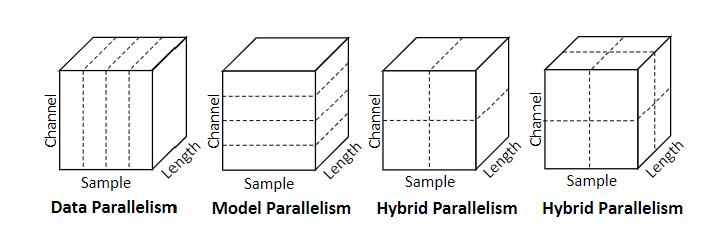
\includegraphics[scale=0.8]{ParallelDimension}
  \caption{Different Spatial Partition Parallelism Strategies}
  \label{fig:paralleldimension}
\end{figure}
 Real word machine learning applications are usually very large, they require tremendous amount of data for training and can not work on a single device. As a result, various parallel strategies has been proposed for running large models in parallel among multiple distributed devices to achieve optimal performance\ref{fig:paralleldimension}. There are different kinds of parallelism strategies, the most common one is Data parallelism\cite{krizhevsky2012imagenet}, where we split input across multiple devices and maintain the same network weight. Data parallelism is adopted and developed by most modern machine learning framework (TensorFlow\cite{abadi2016tensorflow}, Pytorch\cite{paszke2019pytorch}). Data parallelism requires network weight synchronizations between devices at the end of each iteration, therefore Data parallelism is ideal for computation intensive network with few weight parameters (convolution and pooling layer) but will introduce significant communication overhead for network with large number of weight parameters (fully-connected layer). Model parallelism\cite{dean2012large} is achieved by splitting the network weight tensor across devices while broadcast the input tensor. Model parallelism reduces the communication overhead of Data Parallelism but is rarely used because there are often dependencies between network layers. Attribute parallelism\cite{jia2019beyond} can partition the attribute dimension in both input and weight parameter and require collective communication like AllReduce between operations. Experienced developer can combine different Parallelism strategies to achieve optimal performance. For example, \cite{krizhevsky2014one} uses data parallelism for convolution layer and model parallelism for fully-connected layer. All the above parallelism strategies can be categorized as Spatial Partition because they are based on partition on data/weight/operation. \par
   Different from Spatial Partition where input data/weight is distributed across multiple devices, there is another parallelism strategy: Pipeline Parallelism. Pipeline Parallelism divides a machine learning model into several modules with data dependency between them, divides a batch into several micro batches and runs them in parallel in a pipelined fashion. Both GPipe\cite{huang2019gpipe} and Pipedream\cite{narayanan2019pipedream} studied and developed Pipeline parallelism. Pipeline parallelism is especially useful when the training model is too big to fit inside a single device and there are dependencies between different layer. \par
 As shown in \cite{krizhevsky2014one}, combining different parallelism strategies can achieve better performance than only using one strategy. However there is no unifying machine learning framework that can support all the parallelism strategies. TensorFlow\cite{abadi2016tensorflow} and Pytorch\cite{paszke2019pytorch} only supports Data Parallelism while GPipe\cite{huang2019gpipe} and Pipedream\cite{narayanan2019pipedream} supports Pipeline parallelism. User are limited to only a subset of Parallelism strategies, and can not fully utilize the distributed training system. Different distributed system topologies also would require different strategies for optimal performance. As we mentioned before, Spatial Partition may introduce frequent tensor communication overhead between operations. This overhead maybe negligible for a GPU Cluster with high-bandwith inter connections but will definitely cause significant performance drop for large distributed systems consist of several nodes of GPU cluster with low bandwith connection between them. Because high bandwith inter-GPU connection technique like NV-Link can only scale to a limited number of devices, large training server are often deployed across mutiple nodes. It will be ideal to divide the model into several modules and assign each module into a cluster, use Spatial partition inside a GPU cluster and adopt pipeline parallelism for modules across different clusters. In conclusion, a unifying framework that supports all the Parallelism strategies will give user more flexibility and opportunity to achieving optimal performance for training large-scale network across distributed systems for different models and system topologies, and give developer deeper insight into parallel training design.\par
 AIRCoP \cite{aircopfeiwang} is the first framework that supports all the parallel parallelisms above thus allows users to fully explore different parallel settings. AIRCoP implemented spatial partition before and our work implemented Pipeline parallelism for AIRCoP, thus make AIRCoP the first unifying parallel training framework.\par
 \begin{figure}[htbp]
  \centering
  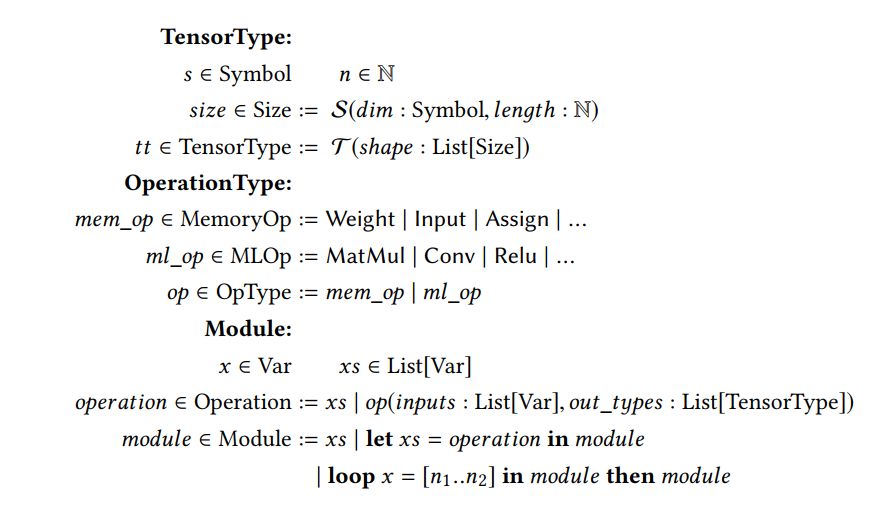
\includegraphics[scale=0.7]{FormalSyntax}
  \caption{Formal Syntax of AIRCoP}
  \label{fig:sample}
\end{figure}
 AIRCoP developed a formal syntax to represent tensor computation graph\ref{fig:sample}. The syntax mainly has 3 components: Tensor and corresponding TensorType to represent input tensor and weight, Operation and corresponding Operation Type to represent different Machine learning operations like Conv/MatMul/Relu and their input/output Type, Module to represent different modules. Operation and Modules are connected through let-bindings. And we use annotation of the formal syntax as an approach to formally represent different parallelism strategies. We developed annotation systems for both Tensor, Operation and Modules. Tensor and Operation annotation represent Spatial Partition by indicating the dimension to partition. Module annotation indicates how many micro-batches the mini batch is split into. Data parallelism can be achieved through annotate the input tensor indicating which dimension to split. Model parallelism can be achieved by annotating the weight tensor. Attribute parallelism can be achieved by a combination  of tensor annotation and operation annotation. And pipeline parallelism can be simply done by annotation the Modules. User only need to write the sequential forward pass of the Machine Learning model and the correct final training loop will be automatically computed through a series of transformation.
 \section{Pipeline Parallelism}
 Pipeline Parallelism is ideal for distributed training workload across several nodes with weak inter-connection. Simply using Spatial Partition across different nodes will cause significant communication overhead between each operation. By splitting the training models into several modules and assigning each modules to different nodes will limit the inter-node communication to the boundary of each module, therefore significantly reduce the inter-node communication overhead.\par
 \begin{figure}[htbp]
  \centering
  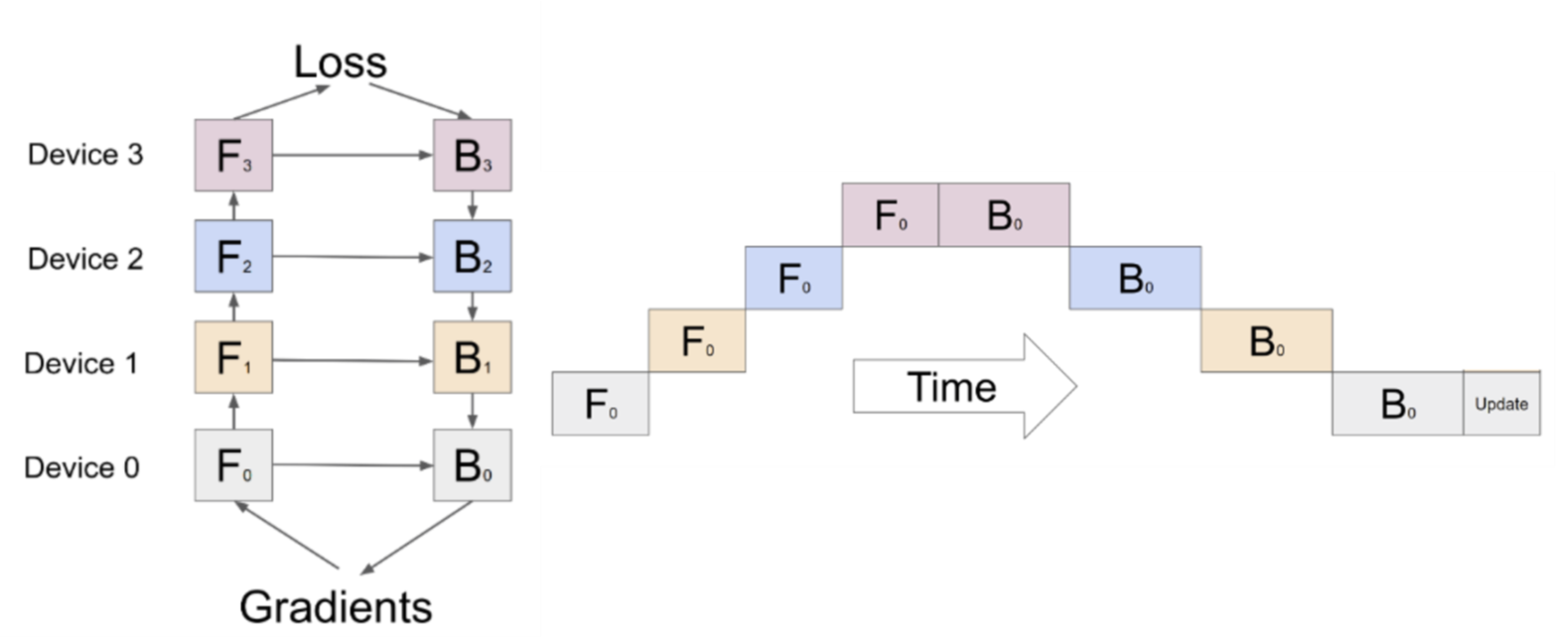
\includegraphics[scale=0.5]{NormalPipeline}
  \caption{Naive multiple modules}
  \label{fig:multiplemodule}
\end{figure}
 Simply splitting modules will cause large amount of stall time (or bubble time) due to complex dependencies between the sequential modules. As shown in\ref{fig:multiplemodule}, if we naively spilt the model into 4 modules $m_0,m_1,m_2,m_3$. There will be sequential dependencies between the forward pass $F_0, F_1, F_2, F_3$ of modules $m_0,m_1,m_2,m_3$, and reverse dependencies between backward pass $B_3, B_2, B_1, B_0$. The dependencies between the forward pass and backward pass will force strict ordering between modules, introduce synchronizations between module boundaries, and cause significant idle time on 4 devices. \par
 \begin{figure}[htbp]
  \centering
  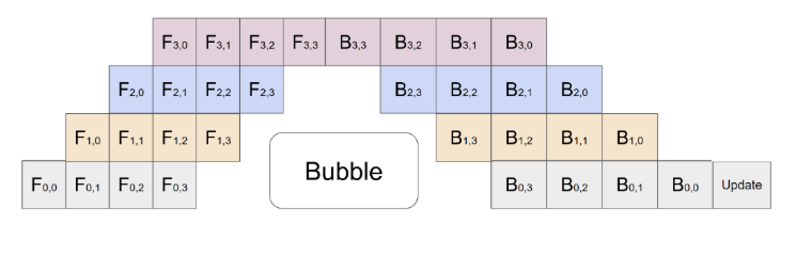
\includegraphics[scale=0.7]{stackedpipeline}
  \caption{Naive multiple modules}
  \label{fig:stackedpipeline}
\end{figure}
 Our approach is similar to GPipe\cite{huang2019gpipe}, we split a batch into multiple micro-batches and run the forward pass and the backward pass of multiple micro-batches sequentially. Only the forward pass and backward pass of the same micro batches has dependencies between them. Different module of different micro-batches could run in parallel as shown in\ref{fig:stackedpipeline}. Pipeline parallelism could allow user to fully utilize distributed devices by minimizing stall time caused by cross-module dependencies. \par
 Pipeline parallelism will insert blocking send/recv operations at the module boundaries to insure necessary execution ordering. And the gradient of multiple micro-batches will be accumulated after all the micro-batches finish and updated the weight synchronously for the entire mini-batch. Pipeline parallelism can easily scale to large number of devices while maintain ideal utilization of resources.\par
 Pipeline parallelism will introduce little communication overhead because it will only transfer data at the module boundaries rather than the frequent inter-operation tensor communication introduced by Spatial Partition. This feature of Pipeline parallelism makes it suitable not only for high-speed inter-connection system but also weakly connected systems. \par
 Pipeline parallelism in AIRCoP is done through module annotation systems. The annotation consists of a integer representing the number of micro-batches (or pipelines). User can splitting the model into several modules and annotates them for Pipeline parallelism. The resulting training loop is slightly different from naive multiple modules. Assume we have $n$ pipelines, the target program will have a top-level training loop for iterating mini-batches. Inside each mini-batch iteration, there will be a training loop of size $n$ for iterating the forward pass of the $n$ micro-batches and a training loop of size $n$ for iterating the backward pass of the $n$ micro-batches. The gradient will be accumulated inside each backward pass of micro-batches. After the backward pass training loop finishes, the weight will be updated based on gradient decent for the entire mini-batch.
 \section{Implementation}
 We implement AIRCoP and Pipeline Parallelism in LMS compiler framework\cite{rompf2010lightweight}, and generate CUDA\cite{sanders2010cuda} code with MPI\cite{gropp1999using}/NCCL for communication as the target executable program.\par
  LMS (Lightweight Modular Staging) is a library-based staging compiler that distinguish stages solely based on Type information. LMS is extremely useful for developing DSL through overloading. It has a typed frontend making the code generation safe. LMS offers lifted (next-stage) version of normal operators and normal control-flow statements makes symbolic code generation easily and convenient. AIRCoP is simply a tensor computation DSL embedded inside LMS framework.\par
 We embedded the formal syntax of AIRCoP inside the IR of LMS. LMS has ANF\cite{flanagan1993essence} form sea of Nodes\cite{click1995simple} IR. It also has a effect system for dealing with side effects and dependencies introduced by effects. LMS can perform Dead Code Elimination and Common Subexpression Elimination, make it sufficient for our tensor computation graph transformation. LMS IR is customizable and offers user flexibility to define their own operation while maintain the data and effect dependencies between them. We use custom IR nodes to represent Input/Weight Tensor and Machine learning Operations, and using the effect system to represent their dependencies. The Module can be simply represented by a Node with a block which contains all of its operations. \par
 The typed frontend source language of AIRCoP only contains the sequential forward computation of the model and annotations. The source language does not mutate tensors. We use overloading of the typed frontend objects and operations and reflection to generate the corresponding IR of the source program. We put the explicit TensorType and Annotations into the rhs of the IR to make it persistent and used in later transformation. \par
 We use transformation pass of LMS to transform the IR and simulate the tensor graph transformation to generate the correct training loop. We first need to perform DimName pass to merge the equivalent dimension of different tensors. For example, if matrix multiplication happens between matrixes of dimension $[m, n]$ and dimension $[j,k]$, then dimension $n$ and dimension $k$ can be merged.  Annotations of tensors and operations represent which dimension to partition, so we have to update those annotations as well. \par
The next pass DistributeTensorAIRCoP is the core pass to implement training loop transformation. This pass has 2 phases \textbf{Collection Phase} and \textbf{Generation Phase}.\par
 The \textbf{Collection Phase} collects the forward operations, the weight nodes and the corresponding backward operation of each node. The backward operation is collected in reverse order to maintain the correct semantic of differentiation. After Collection Phase, we have the necessary information needed to perform automatic differentiation (AD). To generate the correct training loop, we also need to collect lifted tensors. As we mentioned before, the forward pass and backward pass of micro-batches are iterated in different loops to achieve pipeline parallelism. Therefore, the tensors that are allocated in the forward pass and used in the backward pass will cause error because forward and backward pass are now in different scope. Those tensors are called lifted tensors, we have to lift them into the outer scope and maintains multiple versions of them as an array of tensors. The forward and backward pass of micro-batches will use different versions of them lifted tensors. After collect the lifted tensors, the Collection Phase is finished.\par
 The \textbf{Generation Phase} generates the correct training loop based on the collected information. It will add paired send/recv operations at the boundaries of different modules to maintain the correct data dependencies. Inside each module, it will first generates the top-level training loop for mini-batches. Then it will generate the forward training loop and backward training loop for micro-batches based on Module Annotations and use the collected backward operations to realize automatic differentiation. Inside both the forward and backward pass, the read and write to the lifted tensors will be transformed into read/write to the versioned tensor array. The weight gradient will be accumulated in the backward pass and optimized in the end for the entire mini-batch.\par
 The next pass will perform the Spatial Partition transformation. This part is of past work so we will not dig further into this pass. The main purpose of this pass is to partition the tensor and operations based on annotations and add the corresponding inter operation tensor communication for synchronization (AllReduce for MatrixMultiplication or Convolution).\par
 The final pass is to generate the corresponding MPI/NCCL instructions for inter-device communications. NCCL (NVIDIA Collective Communications Library) is the communication library introduced by NVIDIA for efficient collective and point to point communication across multiple GPU and multiple Nodes. Our target program is CUDA code with MPI/NCCL for communication, we use MPI to set up the environment and the NCCL communicator. We will create 2 NCCL communicator, one global communicator for cross-module communication (NCCLSend/Recv) and one local communicator for collective tensor communication (NCCLAllReduce) inside modules. We also need to handle tensor communication between modules if they have different partitions which can be naively implemented by gather and scatter. We use cuBLAS and cuDNN for matrix computation and convolution network. To optimize the memory management, we statically allocate GPU memory before training loop and avoid time-exhausting cudaMalloc/cudaFree inside training loop. \par
 Our generated CUDA code can efficiently represent the correct training loop of machine learning model with both Spatial Partition and Pipeline Parallelism.
 \section{Evaluation}
 In this section we show the evaluation benchmarks of various forms of Pipeline parallelism by running our generated CUDA code on 4 GeForce TITAN XP GPUs. We did not perform comparison between Spatial Partition and Pipeline parallelism because the ideal network topologies for Pipeline parallelism is a large training system consist of several sever Nodes which we do not currently have. The purpose of this benchmark is to validate our graph transformation and gain a deeper insight into the choice of different parallelism strategies.\par
 We perform our test on a micro benchmark (10 convolution layer network) with different parallelism settings:
 \begin{itemize}
   \item Naive 2 module parallelism with each module running in Data parallelism on 2 GPUs
   \item 2 modules in Pipelined parallelism (4 pipelines) with each module running in Data parallelism on 2 GPUs
   \item 2 modules in Pipelined parallelism (8 pipelines) with each module running in Data parallelism on 2 GPUs
   \item 4 modules in Pipelined parallelism (4 pipelines) with each module running in a single GPU
 \end{itemize}
 \begin{figure}[htbp]
  \centering
  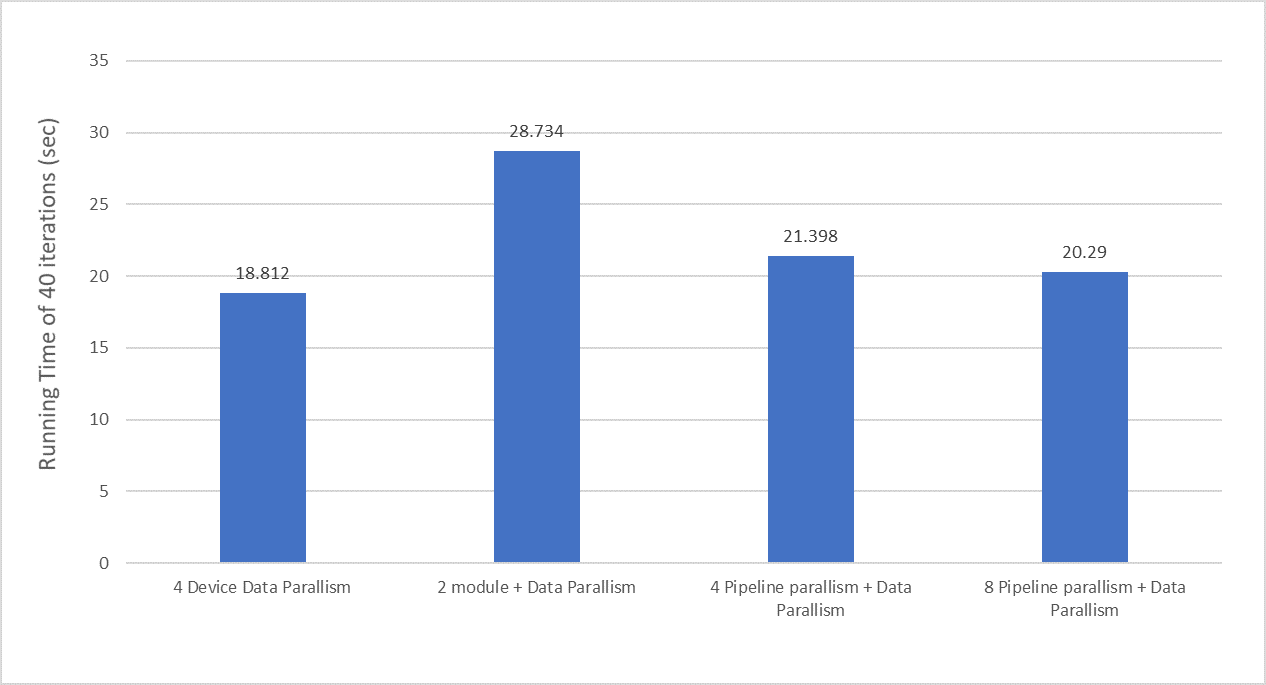
\includegraphics[scale=0.4]{runtime.png}
  \caption{Data Parallelism vs Pipeline parallelism}
  \label{fig:runtime}
\end{figure}
 All the 4 settings runs in 4 GPUs and the running time of 100 iterations on these settings are shown in figure\ref{fig:runtime}. We can notice that using Pipelined parallelism rather than naive module partition on 2 modules will cause a speed up of 1.4x. And we can further accelerate the training loop by either increase the pipeline number (micro-batch number) or the module number. But keep in mind that increase pipeline number will increase memory usage due to versioned tensor and increase module number will increase cross-module communication overhead.\par
 The speed up achieved may not seem significant but is understandable due to the fact that the communication (NCCLSend/Recv) is blocking and could take considerable time for large data transfer. Load in-balancing between different modules could also cause performance drop.\par
 The evaluation shows that our framework can unify both Spatial Partition and Pipeline Parallelism, validates the correctness of our training loop transformation and offers a deeper insight into how to choose between different parallelism training settings.
 \section{Conclusion}
In conclusion, we implement Pipeline parallelism for AIRCoP, make it the first machine learning framework to integrate all the parallelism strategies and offer user flexibility to fully explore different combinations of parallel training strategies under different hardware scenarios and gain a deeper insight into parallel training.
\bibliographystyle{acm}
\bibliography{paper}
\end{document}
\endinput
